\section{Experiments}
\label{sec:experiments}

In this section we present an experimental evaluation of SCORE's performance on
several RA-SLAM problems, consisting of (1) three real-world trials
involving an autonomous underwater vehicle (AUV) and acoustic beacons, (2)
simulated single-robot experiments with a single static beacon, and (3)
simulated multi-robot scenarios with inter-robot ranging. These experiments were
chosen to
respectively demonstrate (1)
SCORE's utility in real-world settings, (2) the challenge of RA-SLAM in even
seemingly simple cases (single-robot and single-beacon), and (3) SCORE's
performance in the challenging, but useful, scenario in which the relative
transformation between robots must be estimated from odometry and range
measurements.

We compare initialization techniques by obtaining an initialization, locally
optimizing the initialization according to Prob. \ref{prob:ra-slam-nls} and
then evaluating the final, locally refined estimates. All comparisons involved a
single initialization and a single local optimization, as opposed to iteratively
re-optimizing as new measurements are added.
Our SCORE implementation
follows \cref{sec:score-to-initialize}, using Drake \cite{drake}
and the Gurobi convex solver \cite{gurobi}.

We emphasize that the initialization strategies compared against represent
either ideal scenarios (ground truth values) or the existing
state-of-the-art (odometric approaches) for the problems presented in these
experiments. Whereas sophisticated initialization techniques exist for
pose-graph SLAM problems, RA-SLAM lacks such techniques.

Quantitative analysis was in comparison to ground truth values and was based on
absolute pose error (APE) \cite{grupp2017evo}.

\subsection{Real-World AUV Experiments}

The AUV data was collected using four acoustic beacons and a Bluefin Odyssey III
off the coast of Italy.  As GPS was not available for most of the collection, we
obtained ground truth AUV positioning via MAP estimation, using GPS for the
initial pose and combining odometry and acoustic ranging with known beacon
locations to localize the remaining trajectory. Ground truth beacon positions
were obtained by surveyed acoustic trilateration prior to the experiment. We
obtained odometry measurements by estimating speed from Doppler velocity log
(DVL) measurements and combining the speed estimate with heading from the INS
magnetometer. We extracted range measurements via two-way time-of-flight ranging
with the acoustic beacons.

\SingleRobotGoatsTrajectoryFigure
\SingleRobotGoatAPEBarPlot

\subsubsection{Single-Robot Odometry Initialization (Odom)}
\label{sec:single-robot-odom-init}

The Odom initialization set the first pose to be the identity matrix and used
composition along the (noisy) odometry chain to obtain the remaining poses. The
static beacon initialization uses a random sample drawn from the environment, as
done in standard techniques \cite{Newman03icra,guo2017ijmav}.

\subsubsection{Evaluation of Single-Robot Experiments}

As seen in \cref{fig:single-robot-trajs}, the SCORE initialized solution closely
matched the ground truth trajectory. The APE results in
\cref{fig:single-trajectory-error} support this argument, showing consistently
lesser APE for the SCORE initialized solution in comparison to the Odom
solution.

\subsection{Generation of Simulations}
\label{sec:generation-simulated-experiments}


We simulated RA-SLAM problems in which robots moved along a grid and
measurements used the noise models of \cref{sec:noise-models}. In all simulated
trials the initial position of any robots or beacons were randomly placed within
the simulated environment. At each time step odometry measurements were recorded
for each robot and each robot had a 50\% chance of generating a range
measurement. If generated, the remaining endpoint of the range measurement was
chosen by uniform sampling from the set of all other robots and beacons present.

\SingleRobotTrajectoryFigure
\SingleRobotAPEBoxPlot

To evaluate the effect of different sensor noise levels, we tested low- and
high-noise cases for both the single-robot and multi-robot scenarios. Each set
of noise parameters comes from values found in previous real-world experiments.
All odometry measurements were 1-meter movements, so a standard deviation of
0.01 meters in translation measurements corresponds to 1\% of the distance
traveled.

The low-noise setting uses $\sigma^{2}_{ij} = \lowSigmaSq$, $\tau^{-1}_{ij} =
\lowTauInv$, and $\kappa^{-1}_{ij} = \lowKappaInv$. This corresponds to standard
deviations of $\lowSigma$ meters, $\lowTauInvSqrt$ meters, and 0.002 radians
(0.41 degrees) for distance, translation, and rotation measurements,
respectively. The high-noise setting uses $\sigma^{2}_{ij} = \highSigmaSq$,
$\tau^{-1}_{ij} = \highTauInv$, and $\kappa^{-1}_{ij} = \highKappaInv$.


\subsection{Simulated Single-Robot Experiments}
\label{sec:single-robot-experiments}

In this section we evaluate the single-robot experiments, which considered
single robot and single static ranging beacon. For both the high and low noise
cases we generated 20 trials, with each trial consisting of 400 poses. For each
trial we compare the results of three different initialization strategies:
SCORE, simple odometry composition, and GT-Init (in which the ground-truth is
used as initialization).

\subsubsection{Evaluation of Single-Robot Experiments}

As seen in \cref{fig:single-robot-trajs}, the SCORE initialized solution
appeared to exactly match the GT-Init initialized solution. This is supported by
the quantitative results in \cref{fig:single-trajectory-error}, which suggest
that SCORE and GT-Init initialization effectively resulted in the same APE for
the trials run. In contrast to SCORE and GT-Init, the Odom initialization
obtained notably worse solutions (i.e. substantially higher APE and
qualitatively incorrect).  In \cref{fig:single-trajectory-error} it can be seen
that the Odom initialization resulted in an increase in APE of up to two orders
of magnitude.

\subsection{Multi-Robot Experiments}
\label{sec:multi-robot-experiments}

\MultiRobotTrajectoryFourPanelFigure

To test a scenario in which initialization is difficult, we
simulated scenarios with four robots and no ranging beacons. For both the high
and low noise cases we generated 20 trials with 400 poses per robot (1600 poses
per trial). We compare the results of four different initialization strategies:
SCORE, ground truth (GT-Init), odometry with perfect first pose (Odom-P), and
odometry with random first pose (Odom-R). We describe these approaches in detail
in \cref{sec:multi-robot-init}.

\subsubsection{Multi-Robot Initialization}
\label{sec:multi-robot-init}

GT-Init is an idealistic case in which the ground truth state is known \textit{a
priori} and all variables are initialized to their true values. While RA-SLAM is
not needed if the true state is known, GT-Init is meant to serve as an upper
bound for reasonable quality of an initialization technique.

In comparison to the GT-Init initialization, the odometry based initializations
represent more realistic scenarios in which either the initial pose of each
robot is known (Odom-P) or no prior information exists (Odom-R). Odom-P and
Odom-R only differ in choosing the starting pose for each robot. After
determining the starting pose for a given robot both Odom-P and Odom-R compose
odometry measurements to initialize the remaining poses for all robots.

In Odom-P we assume a perfectly known starting pose of each robot and compose
the odometry chain to initialize the other pose variables. Such a situation may
occur in marine robotics, where AUVs begin with GPS before diving underwater.
In contrast to Odom-P, for Odom-R we assume no prior information and choose the
starting pose for each robot randomly. Odom-R is a standard
approach to initialization for multi-robot RA-SLAM \cite{guo2017ijmav,li20arxiv}
and is arguably the fairest comparison for SCORE as both require no prior
information.


\subsubsection{Evaluation of Multi-Robot Experiments}

As seen in the example multi-robot trial displayed in
\cref{fig:multi-robot-trajs}, SCORE provides reliable estimates of the
trajectories of the four robots. In this trial the solution obtained from the
SCORE initialization qualitatively matches the true trajectories. In addition,
the refined SCORE initialization appears to match the trajectories estimated
using the GT-Init initialization and provide a substantially better estimate
than that provided by the Odom-P and Odom-R initializations.

These qualitative observations from \cref{fig:multi-robot-trajs} are supported
by the APE evaluation in \cref{fig:multi-trajectory-error}. We
observe that for the high-noise multi-robot experiments the SCORE initialization
strategy resulted in similar APE to the GT-Init initialization and had
reduced APE in comparison to Odom-P and Odom-R. For the low-noise multi-robot
experiments SCORE resulted in higher APE than the GT-Init initialization
approach but lesser APE than either of the odometric initialization strategies.

\MultiRobotAPEBoxPlot


\subsubsection{Runtime Evaluation}
\label{sec:runtime-evaluation}

\begin{figure}[!tp]
    \begin{center}
        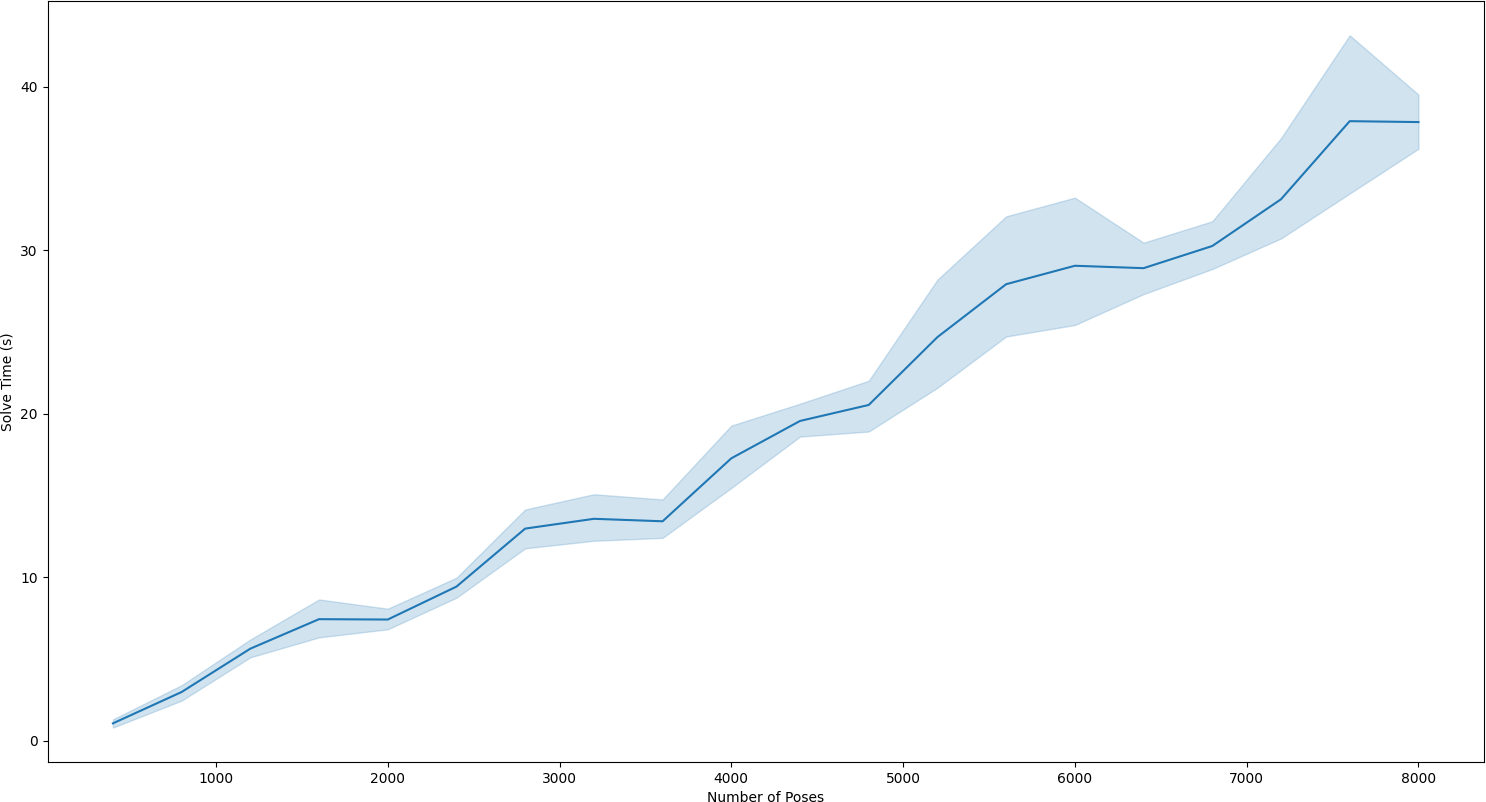
\includegraphics[width=\linewidth, trim={0mm 0mm 0mm 0mm},clip]{figures/score_runtimes_confidence-trimmy.png}
    \end{center}
    \vspace{-2mm}
    \caption{Time to solve SCORE problems of increasing size. The solid
    line indicates the mean, with the shaded region indicating a 95\%
    confidence region. Statistics were computed from 10 experiments at
    each problem size.}
    \label{fig:runtime-evaluation}
    \vspace{-4mm}
\end{figure}

To evaluate the scalability of SCORE we solved multi-robot RA-SLAM problems of
increasing size. The problems were four-robot problems with six static beacons
and robot-robot and robot-beacon ranging. The problem size ranged from 100 poses
per robot (400 poses total) to 2000 poses per robot (8000 poses total), and grew
in increments of 100 poses per robot (each subsequent trial grew by 400 poses
total). Each robot had 10\% chance of generating a range measurement at each
time step. Each robot had its own odometry chain, but there were no pose-pose
measurements between differing robots. For each problem size, 10 random
experiments were generated.

The results of these experiments can be seen in \cref{fig:runtime-evaluation},
which displays the time required to solve the SCORE problem. As can be seen,
there is a clear consistent increase in solve time as the problem grows, though
there is some variation in the solve times at each size. Importantly, while not
able to run in real-time, these experiments demonstrate that SCORE can solve
problems of meaningful size in reasonable time for real-world applications.
Depending on the specific application, SCORE could be run periodically to update
an RA-SLAM solution after many new measurements were collected.
